\chapter{Introduction}
    The aim of this project is design and implementation of hearth rate and oxygen saturation monitor.
    Hearth rate frequency (measured in beats per minute) as well as oxygen saturation needs to be shown on display. \\
    Used components were:
    \begin{itemize}
        \item \texttt{MAX30102} sensor of hearth rate and oxygen saturation \cite{max30102:manual}
        \item \texttt{SSD1306} OLED display \cite{ssd1306:manual}
        \item \texttt{ESP32} microcontroller \cite{ESP:Manual}
    \end{itemize}
    From software's point of view, the heart is \texttt{Espressif IoT Development Framework}\cite{espidf:docs} \texttt{(ESP-IDF)}. 
     
\chapter{Circuit diagram, components}
    To easier manipulation, every components is placed on breadboard but for illustration purposes, components are connected directly.\\
    \begin{figure}[ht!]
    \centering
    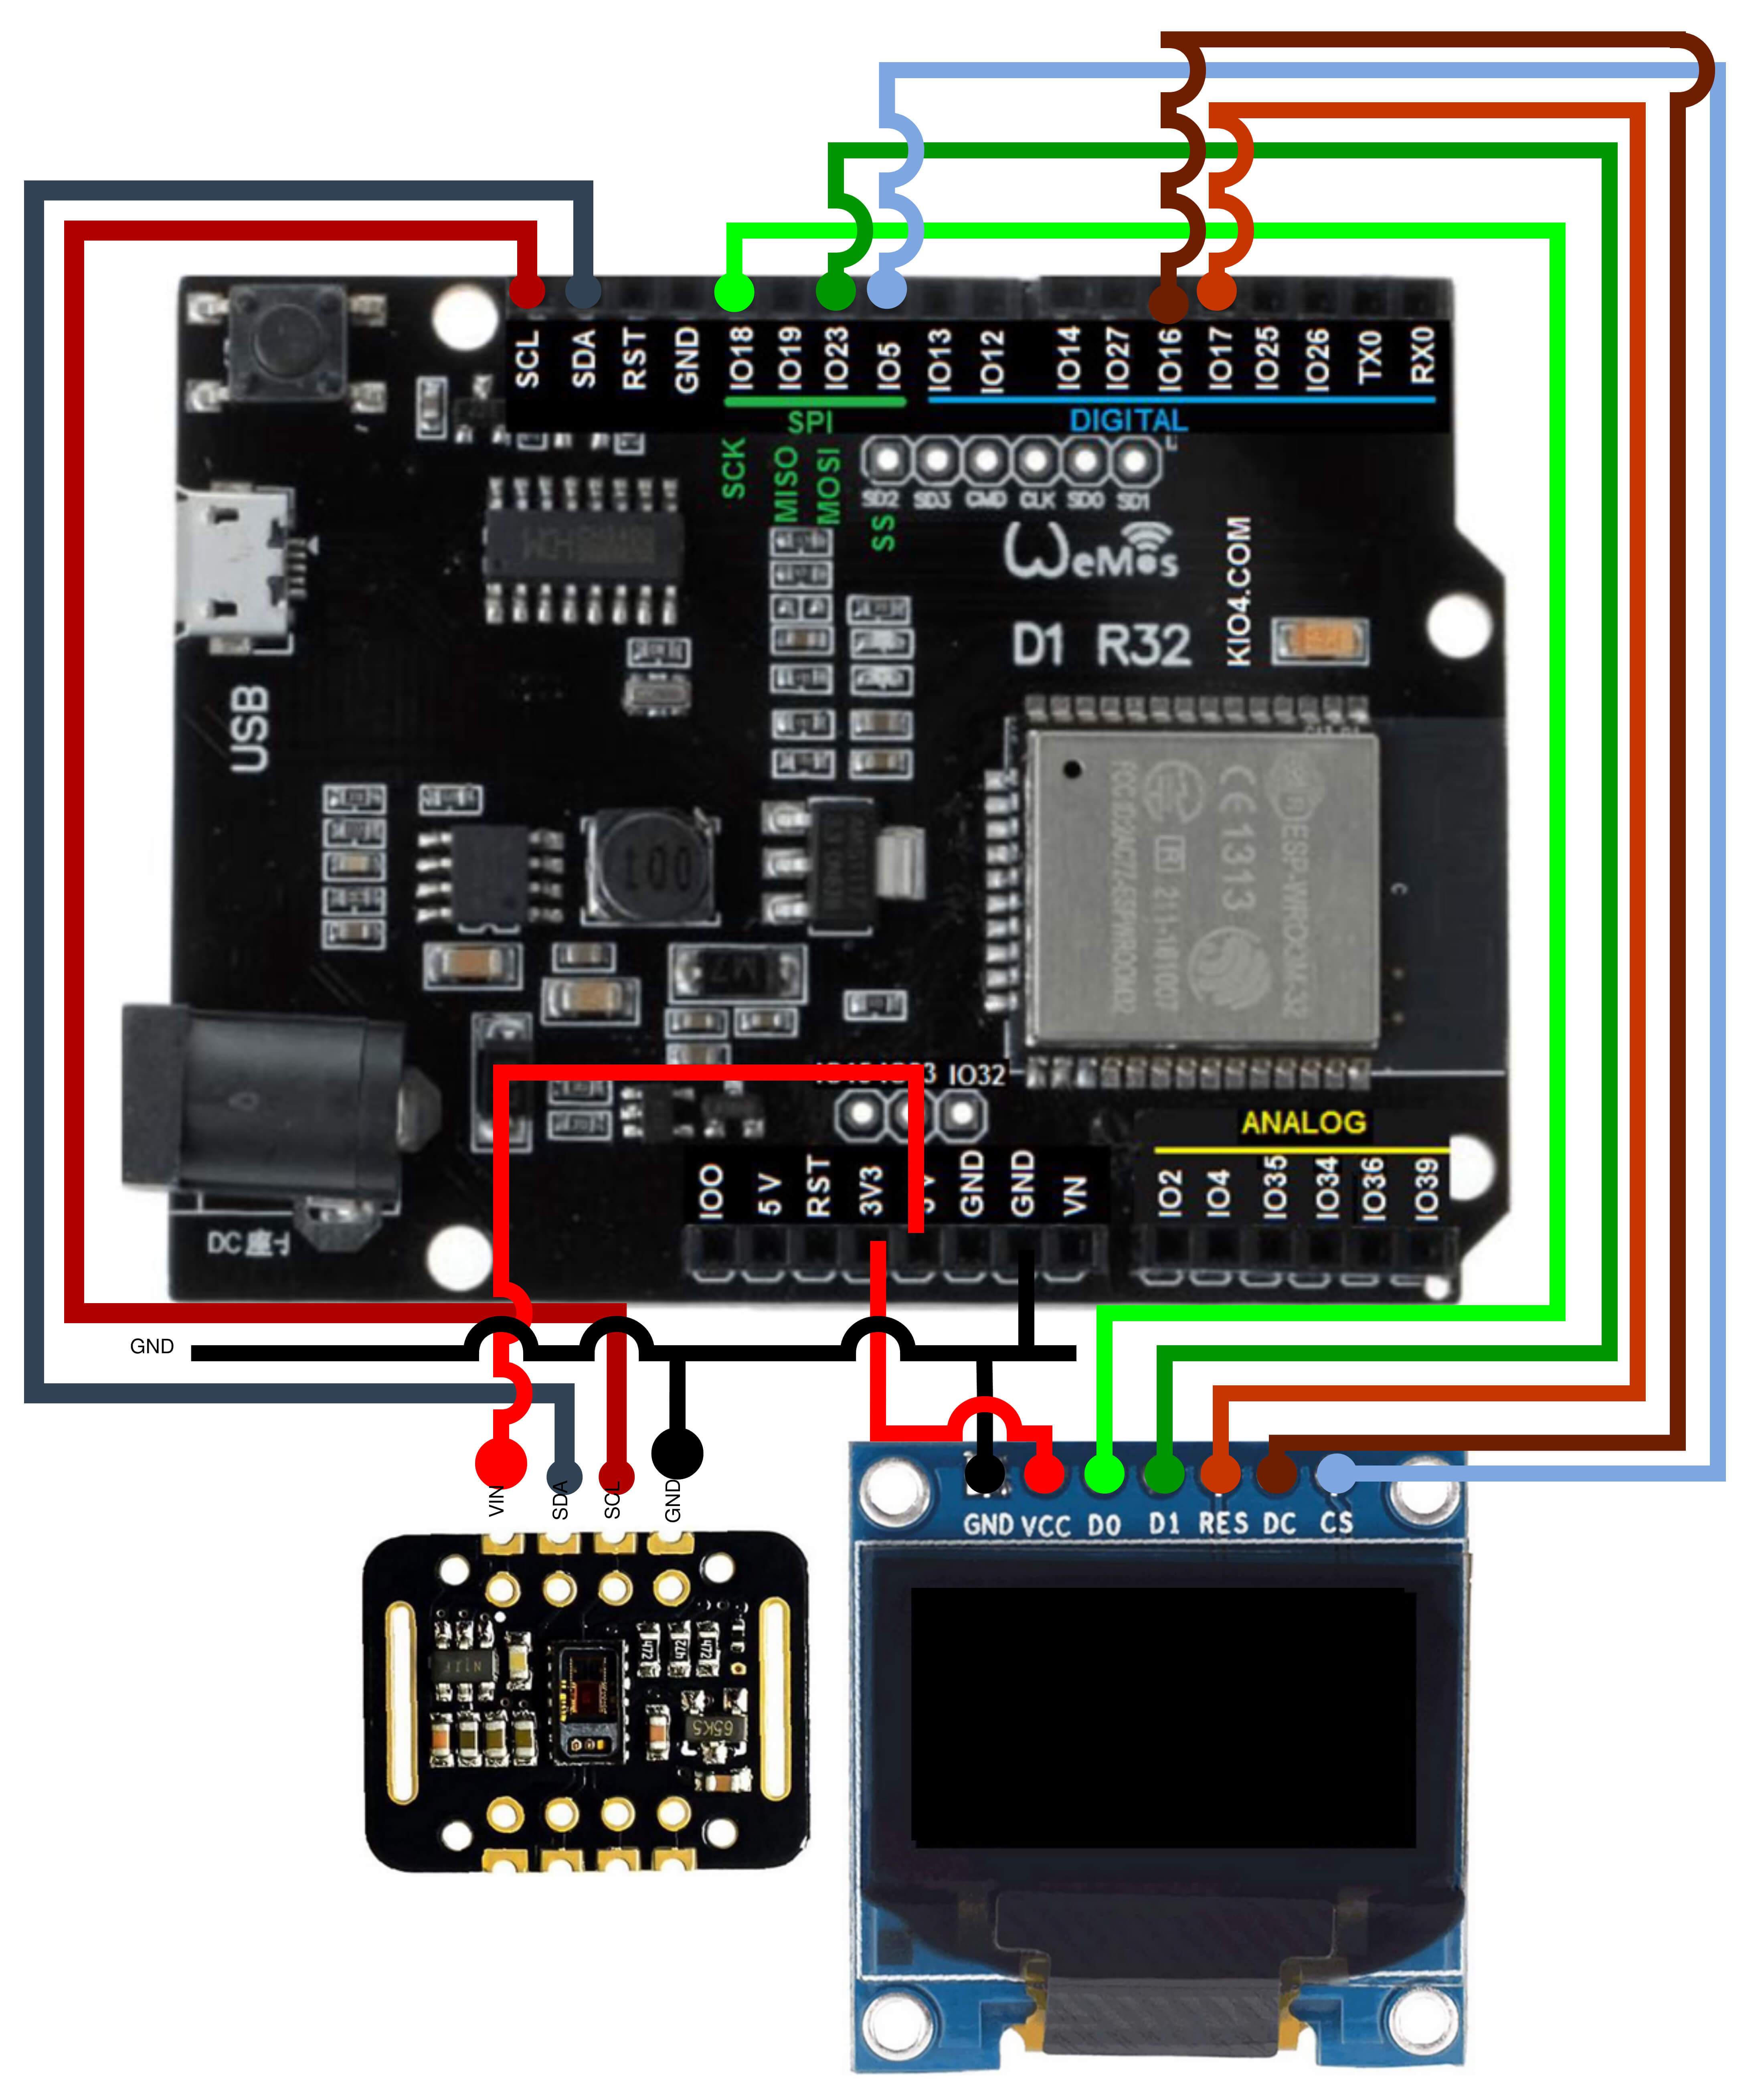
\includegraphics[width=90mm]{scheme.jpg}
    \caption{Circuit diagram}
    \end{figure}

    \section{\texttt{MAX30102} - pulse oximeter}
    \label{max30102}
        Module uses \texttt{$I^2C$}\footnote{More on \href{https://en.wikipedia.org/wiki/I\%C2\%B2C}{https://en.wikipedia.org/wiki/\texttt{$I^2C$}}} protocol for communication with outside components. \\
        Input voltage pin of oximeter is connected to $5V$ pin on \texttt{WeMoS} board. For grounding, common ground both for display and oximeter is used. Since this sensor uses \texttt{$I^2C$} for communication, pins \texttt{SDA} and \texttt{SCL} are connected to the same pins on microcontroller - \texttt{SDA} and \texttt{SCL}.
    \section{\texttt{SSD1306} OLED display}
        Display support both \texttt{$I^2C$} and \texttt{SPI}. But since \texttt{$I^2C$} is already used for \nameref{max30102} \texttt{SPI} needs to be used instead. Display requires $3.3V$ as input voltage, common ground both for oximeter and diplay is used. \texttt{D0} pin is connected to \texttt{I018} pin on microcontroller and \texttt{D1} is connected to pin \texttt{I023}. Data/command (\texttt{DC}) pin is connected to pin \texttt{I016} on the microcontroller side, as well as chip select \texttt{CS} pin is connected to \texttt{I05}. Reset pin \texttt{RST} is connected to \texttt{I017}.
   
\chapter{Implementation}
    Project was inspired by \cite{hackerio}, implementation of \texttt{$I^2C$} communication with pulse oximeter is taken from there as well as algorhitm of proration to beats per minutes. Some parts of this ``library'' was refactored.
    Communication over \texttt{SPI} with text rendering is not implemented from scratch, standard but adjusted \texttt{ESP-IDF} library is used, available on \href{https://github.com/nopnop2002/esp-idf-ssd1306}{https://github.com/nopnop2002/esp-idf-ssd1306}. Some of unnecessary parts were removed.\\
    Rest of the implementation is done in \texttt{main/main.c} file. \\
    

    After machine boot \texttt{app\_main} function is executed. It initializes both display and pulse oximeter. Afterwards $2$ tasks ``parallel'' are created - \texttt{max30102\_task} and \texttt{draw\_data\_task}.
    \texttt{draw\_data\_task} based on global variable \texttt{finger\_on\_sensor} prints ``Put your finger on the sensor'' message. If the finger is placed on sensor, actual hearth rate and oxygen saturation is printed on the display. Those 2 values are updated by \texttt{max30102\_task} task and minimal allowed time between updates is $0.5\ seconds$.

    \subsection{Flashing}
        Program needs to be compiled and flashed to microcontroller. Just use \texttt{idf} and \texttt{idf.py flash monitor} command that builds everything (if necessary) and flashes it into \texttt{ESP32}.

\chapter{Video demonstration}
    Video demonstration of project could be found on \\ \href{https://www.youtube.com/watch?v=KGk2CRs4Ns8}{https://www.youtube.com/watch?v=KGk2CRs4Ns8}.
        
\chapter{Conclusion}
    Project implements all the parts of assignment, it even implements displaying of oxygen saturation. Results are not ``profesionally'' validated, I just compared it with my Apple Watch and results were close to each other.

    \subsection{Proposed evaluation}
        \begin{itemize}
            \item Functionality 5\ pts - project implements all required functionality, there is even displaying of oxygen saturation
            \item Quality of code 2\ pts - project is not implemented from scratch
            \item Presentation 1\ pts
            \item Documentation 3\ pts - scope is not that big
            \item Approach 1\ pts
            \item Total 12\ pts
        \end{itemize}
%=========================================================================
